\noindent \bf{(1)稳定性因素$K$、特征车速$u_{ch}$:}

$$
    K = \frac{m}{L^2}(\frac{a}{k_2}-\frac{b}{k_1})=\frac{1818.2}{3.048^2}(\frac{1.463}{-110185}-\frac{1.585}{-62618})=2.355\times10^{-3} s^2/m^2
$$

$$
    u_{ch} = \sqrt{1/K} = \sqrt{1/(2.355\times10^{-3})} = 20.6 m/s
$$

\noindent \bf{(2)稳态横摆角速度增益曲线$\frac{\omega_r}{\delta})_s-u_a$}

由式(5-11)可知,

$$
    \frac{w_r}{\delta}\big)_s = \frac{u/L}{1+Ku^2}
$$

因此设计Matlab程序:
\begin{lstlisting}[language=Matlab]
    %上题求得的稳定性因数
    K = 2.355*10^(-3);
    %车身长度
    L = 3.048;
    %速度区间设置在1-40m/s
    u = 1:40;
    %横摆角速度增益曲线
    YawRateGain1 = (u/L)./(1+K*u.^2);
    %设置K=0的情况作为对照
    YawRateGain2 = u/L;
    %绘图
    plot(u,YawRateGain1);
    axis([0 40 0 10]);
    hold on
    plot(u,YawRateGain2)
\end{lstlisting}

获得横摆角速度增益曲线如下图所示。

\begin{figure}[h]
    \centering
    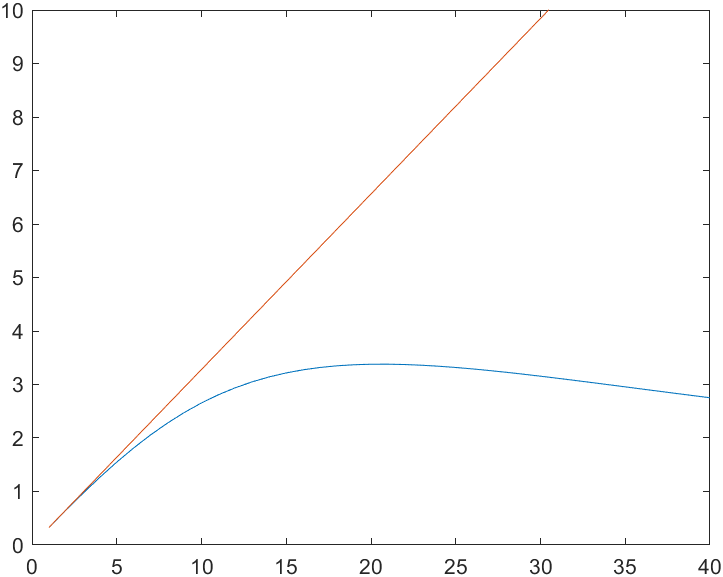
\includegraphics[width=5.5cm]{figure/YRG.png}
    \caption{横摆角速度增益曲线}
    \label{YawRateGainCurve}
\end{figure}

\noindent \bf{(3)车速$u_a=22.35m/s$时的转向灵敏度$\frac{\omega_r}{\delta_{s\omega}}$

根据公式(5-11)计算可得,车速$u_a=22.35m/s$时的稳态横摆角速度增益$\frac{w_r}{\delta})_s=3.37$,
该车的转向系总传动比$i=20$,即$\delta_{s\omega}=i\delta$,所以$\frac{\omega_r}{\delta_{s\omega}}=\frac{\omega_r}{\delta})_s/i=0.1685$

\noindent \bf{(4)静态储备系数S.M.}
由公式(5-17)可得:
$$
    S.M. = \frac{k_2}{k_1+k_2}-\frac{a}{L} = \frac{-110185}{-62618-110185}-\frac{1.463}{3.048} = 0.157
$$
S.M.为正值,汽车具有不足转向特性。

\noindent \bf{(5)侧向加速度为0.4g时的前、后轮侧偏角绝对值之差$\alpha_1-\alpha_2$与转弯半径的比值$R/R_0(R_0=15m)$}
由公式(5-13)可得,
$$
\alpha_1-\alpha_2 = K\times a_yL = 28.13\times10^{-3} rad 
$$

$$
\begin{gathered}
    R_0 = L/\delta = 15m, \\
    \delta = 0.2032 rad \\
    R = \frac{L}{\delta - (\alpha_1-\alpha_2)} = \frac{3.048}{0.2032-0.02813} = 17.41m\\
    \frac{R}{R_0} = \frac{17.41}{15} = 1.16;
\end{gathered}
$$

\noindent \bf{(6)车速$u=30.56m/s$时,瞬态相应的横摆角速度波动的固有(圆)频率$\omega_0$、阻尼比$\zeta$、反应时间$\tau$与峰值反应时间$\epsilon$}

由公式(5-34),(5-35),(5-36),(5-37)得:
$$
\begin{gathered}
    \omega_0 = \frac{L}{u}\sqrt{\frac{k_1k_2}{mI_z}(1+Ku^2)} = 4.62 \\
    \zeta = \frac{-m(a^2k_1+b^2k_2)-I_Z(k_1+k_2)}{2L\sqrt{mI_Zk_1k_2(1+Ku^2)}} = 0.589\\
    \tau = -\frac{arctan[\frac{\sqrt{1-\zeta^2}}{(-\frac{mua}{Lk_2}\omega_0-\zeta)}]}{\omega_0\sqrt{1-\zeta^2}} = 0.2586s\\
    \epsilon = \frac{arctan(\frac{\sqrt{1-\zeta^2}}{\zeta})}{\omega_0\sqrt{1-\zeta^2}}+\tau = 0.467s
\end{gathered}
$$
